\title{Harmonic analysis}

\maketitle
\tableofcontents

\definecolor{violeta}{rgb}{0.5,0.0,1.0}

\section{Harmonic analysis for what?}
\begin{itemize}
\item Harmonic analysis~\cite{Lathi} is a mathematical tool that
  allows expressing a function f (t) in relation to a set of
  orthogonal functions gi (t), by means of a linear combination of
  these. In other words,
  $$
  f(t) = \sum_i a_ig_i(t).
  $$
\item By conveniently choosing the set of orthogonal functions we can
  perform an analysis of $f(t)$ according to the characteristics or
  properties of the functions $g_i(t)$.
\item One of the most frequent practical applications of Fourier
  analysis is the representation of signals according to their
  frequency components. This is achieved because the base functions in
  the harmonic analysis are sinusoids.
\end{itemize}

\section{The Fourier trigonometric series}
\begin{itemize}
\item Any function (or signal) $s(t)$ can be represented by a a linear
  combination of sinosuidal functions.
\item Let $f(t)$ be a function defined in the interval $(t_0,
  t_0+\frac{2\pi}{\omega_0})$. The Fourier trigonometric series allows
  to represent $f(t)$ in terms of the complete orthogonal set of
  sine-wave
  functions~\cite{Oppenheim} \begin{equation*} \begin{array}{ll} \{1;
  & \cos(\omega_0t), \cos(2\omega_0t), \cdots, \cos(n\omega_0t), \cdots;\\
  & \sin(\omega_0t), \sin(2\omega_0t), \cdots, \sin(n\omega_0t), \cdots\} \end{array} \end{equation*}
  through the linear combination (\ref{eq:stf}) \begin{equation} f(t)
  = a_0 + \sum_{n=1}^\infty \big(a_n \cos(n\omega_0t) +
  b_n \sin(n\omega_0t)\big), \tag{stf} \label{eq:stf} \end{equation}
%    \begin{array}{rl}
%      f(t) = & a_0 +\\
%      & a_1\cos(\omega_0t)+a_2\cos(2\omega_0t)+\cdots+a_n\cos(n\omega_0t)+\cdots\\
%      & b_1\sin(\omega_0t)+b_2\sin(2\omega_0t)+\cdots+b_n\sin(n\omega_0t)+\cdots\\
%      = & a_0 + \sum_{n=1}^\infty a_n \cos(n\omega_0t) + 
%      \sum_{n=1}^\infty b_n \sin(n\omega_0t),
%    \end{array}
  where $$t_0<t<t_0+\frac{2\pi}{\omega_0},$$ $\omega_0$ is the fundamental
  frequency component expressed in radians per second and $a_0$, $a_n$
  and $b_n$ are the coefficients of the Fourier trigonometric series.
\item Note that this summation can only reproduce the behavior of a
  function (or a signal) in an interval (of time) equal to
  \begin{displaymath}
    \frac{2\pi}{\omega_0}.
  \end{displaymath}
  As just defined, this interval is equal to the period of the lowest
  frequency component that exists in the signal.
\end{itemize}

%\newpage
\subsection{Fourier coefficients of the trigonometric series}
\begin{itemize}
\item The coefficients of the Fourier trigonometric series express the
  amount of each of the ``pure sinusoidal signals'' that must be added
  together to obtain the analyzed signal.
\item Mathematically, they are calculated as the proportion that
  exists between the energy of the correlation of the signal with the
  respective sinusoidal function (\ref{eq:an}) and the energy of that
  sinusoidal function (\ref{eq:bn}), ie
  \begin{equation}
    a_n=\frac{\displaystyle
      {\color{blue} \int_{t_0}^{t_0+T}f(t)\cos(n\omega_0t)dt}
    }{\displaystyle
      {\color{violeta} \int_{t_0}^{t_0+T}\cos^2(n\omega_0t)dt}
    } \tag{an}
    \label{eq:an}
  \end{equation}
  \begin{equation}
    b_n=\frac{\displaystyle
      {\color{blue} \int_{t_0}^{t_0+T}f(t)\sin(n\omega_0t)dt}
    }{\displaystyle
      {\color{violeta} \int_{t_0}^{t_0+T}\sin^2(n\omega_0t)dt}
    } \label{eq:bn} \tag{bn}
  \end{equation}
  being
  $$
  T=\frac{2\pi}{\omega_0}.
  $$
\item For $n=0$
  \begin{equation*}
    a_0 = \frac{1}{T}\int_{t_0}^{t_0+T} f(t)dt,
  \end{equation*}
  which, as we can see, is the average value of $f(t)$ in the interval
  $(t_0, t_0+T)$. $a_0$ is refered as the direct current component
  or DC (Direct Current) of $f(t)$ in such interval.

\item On the other hand, knowing that
  $$
  \int_{t_0}^{t_0+T} \cos^2(n\omega_0t)dt = \int_{t_0}^{t_0+T}
  \sin^2(n\omega_0t)dt = \frac{T}{2},
  $$
  the Eqs. \ref{eq:an} and \ref{eq:bn} can be also written as
  \begin{equation}
    a_n = \frac{2}{T}\int_{t_0}^{t_0+T} f(t)\cos(n\omega_0t)dt
    \tag{anOK}
    \label{eq:anOK}
  \end{equation}
  and (\ref{eq:bnOK})
  \begin{equation}
    b_n = \frac{2}{T}\int_{t_0}^{t_0+T} f(t)\sin(n\omega_0t)dt,
    \tag{bnOK}
    \label{eq:bnOK}
  \end{equation}
  which is usually the most common in the literature~\cite{Lathi,Oppenheim}.
%\item Finalmente, indicar que la serie trigonom\'etrica indicada en la
%  Ecuaci\'on \ref{eq:stf} tiene la expresi\'on alternativa
%  \begin{equation}
%    f(t) = \sum_{n=0}^\infty c_n\cos(n\omega_0t+\phi_n)
%    \label{eq:stf2}
%  \end{equation}
%  donde
%  \begin{equation}
%    c_n=\sqrt{a_n^2+b_n^2}
%  \end{equation}
%  y
%  \begin{equation}
%    \phi_n = -\tan^{-1}\Big(\frac{b_n}{a_n}\Big),
%  \end{equation}
%  que se consigue realizando los oportunos cambios trigonom\'etricos.  A
%  los coeficientes $c_n$ se les conoce como modulo de
%  Fourier y a los $\phi_n$ como fase de Fourier.
\end{itemize}

\section{The Fourier exponential series}
\begin{itemize}
\item It is a more compact representation of Eq. \ref{eq:stf}, written
  as a function of the complex exponential.
\item Be the definitions
\begin{equation}
\begin{array}{l}
  a_0 = F_0\\
  a_n = F_{n}+F_{-n}\\
  b_n = j(F_{n}-F_{-n}),
\end{array}
\tag{defs\_Fes}
\label{eq:defs_sef}
\end{equation}
where $j=\sqrt{-1}$.

If we substitute these definitions in the Equation \ref{eq:stf},
we get that
\begin{displaymath}
f(t) = F_0 + \sum_{n=1}^\infty \big((F_{n}+F_{-n}) \cos(n\omega_0t) +
   (j(F_{n}-F_{-n})) \sin(n\omega_0t)\big).
\end{displaymath}
\newpage

Multiplying we get to that
\begin{displaymath}
  \begin{array}{r}
    f(t) = F_0 + \displaystyle\sum_{n=1}^\infty \Big(F_{n}\cos(n\omega_0t)+F_{-n}\cos(n\omega_0t) +\\
    jF_{n}\sin(n\omega_0t)-jF_{-n}\sin(n\omega_0t)\Big).
  \end{array}
\end{displaymath}
Operating
\begin{displaymath}
  \begin{array}{r}
    f(t) = F_0 + \displaystyle\sum_{n=1}^\infty \Big(F_{n}\big(\cos(n\omega_0t)+j\sin(n\omega_0t)\big)+\\
    F_{-n}\big(\cos(n\omega_0t) -j\sin(n\omega_0t)\big)\Big).
  \end{array}
\end{displaymath}
Now applying the trigonometric changes
\begin{equation}
  \begin{array}{c}
    e^{jn\omega_0t} = \cos(n\omega_0t) + j\sin(n\omega_0t)\\
    e^{-jn\omega_0t} = \cos(n\omega_0t) - j\sin(n\omega_0t)
  \end{array}
  \tag{e\_sin\_cos}
  \label{eq:e_sin_cos}
\end{equation}
in the previous expression we get that
\begin{displaymath}
  f(t) = F_0 + \sum_{n=1}^\infty \Big(F_ne^{jn\omega_0t}+ F_{-n}e^{-jn\omega_0t}\Big).
\end{displaymath}
By operating with the sign of the variable $n$ and partially undoing
the sum we get to that
\begin{displaymath}
  \begin{array}{rcl}
    f(t) & = & F_0 + \displaystyle\sum_{n=1}^\infty \Big(F_{n}e^{jn\omega_0t}+F_{-n}e^{j(-n)\omega_0t}\Big) \\
    & = & F_0 + \displaystyle\sum_{n=1}^\infty F_{n}e^{jn\omega_0t} + \displaystyle\sum_{n=-1}^{-\infty} F_ne^{jn\omega_0t}.
  \end{array}
\end{displaymath}
Finally, joining the two summations and the term that was left out we have to
\begin{equation}
  f(t) = \sum_{n=-\infty}^\infty F_ne^{jn\omega_0t}.
  \tag{Fes}
  \label{eq:Fes}
\end{equation}
\item The \ref{eq:Fes} equation is known as the Fourier exponential
  series and the $F_n$ as the coefficients of that series.
\end{itemize}

%\newpage
\subsection{The Fourier complex coefficients}
%\section{Los coeficientes de la serie exponencial de Fourier}
\begin{itemize}
\item Using the definitions made in the Expression \ref{eq:defs_sef}
  it is possible to easily find that
  \begin{equation}
    F_n = \frac{1}{2}(a_n-jb_n).\tag{F\_n}
    \label{eq:F_n}
  \end{equation}
\item Substituting this eq. in the expressions \ref{eq:anOK} and
  \ref{eq:bnOK} we get that (\ref{eq:F_n_OK})
  \begin{equation}
  \begin{array}{rl}
    F_n & = \displaystyle\frac{1}{2}\Big(\frac{2}{T}\int_{t_0}^{t_0+T}
    f(t)\cos(n\omega_0t)dt -j\frac{2}{T}\int_{t_0}^{t_0+T} f(t)\sin(n\omega_0t)dt
  \Big)\\
   & = \displaystyle\frac{1}{T}\Big(\int_{t_0}^{t_0+T}
   f(t)\cos(n\omega_0t)dt -j\int_{t_0}^{t_0+T} f(t)\sin(n\omega_0t)dt\Big)\\
   & = \displaystyle\frac{1}{T}\int_{t_0}^{t_0+T}f(t)e^{-jn\omega_0t} dt
  \end{array}
  \tag{F\_n\_OK}
  \label{eq:F_n_OK}
  \end{equation}
\end{itemize}

\begin{comment}
\section{La serie exponencial de Fourier}
\begin{itemize}
\item Fourier tambi\'en demostr\'o que posible representar cualquier
  funci\'on $f(t)$, definida en el intervalo $(t_0, t_0+T)$, mediante
  una combinaci\'on lineal de funciones exponenciales tal y como se
  muestra a continuaci\'on
  \begin{equation}
    \begin{array}{rl}
      f(t) = & F_0 +\\
      & F_1e^{\omega_0t}+F_2e^{2\omega_0t}+\cdots+F_ne^{n\omega_0t}+\cdots\\
      &
      F_{-1}e^{\omega_0t}+F_{-2}e^{2\omega_0t}+\cdots+F_{-n}e^{n\omega_0t}+\cdots\\
      = &\displaystyle\sum_{n=-\infty}^\infty F_ne^{jn\omega_0t},
    \end{array}
    \tag{}
    \label{eq:sef}
  \end{equation}
  donde $\omega_0=\frac{2\pi}{T}$ es la componente de frecuencia
  fundamental y
  $$
  e^{j\omega_0t} = \cos(\omega_0t) + j\sin(\omega_0t),
  $$
  siendo $j=\sqrt{-1}$.
\newpage
\item Los distintos coeficientes de la serie exponencial de Fourier se
  determinan mediante
  $$
  \begin{array}{rl}
  F_n & =\frac{\displaystyle
    \int_{t_0}^{t_0+T}f(t)(e^{jn\omega_0t})^\star dt
  }{\displaystyle
    \int_{t_0}^{t_0+T}e^{jn\omega_0t}(e^{jn\omega_0t})^\star dt
  }
  \\
  \multicolumn{2}{l}{\text{(Teniendo en cuenta que $e^{-x} = \cos(x)-j\sin(x)$)}}
  \\
  & = \frac{\displaystyle
    \int_{t_0}^{t_0+T}f(t)e^{-jn\omega_0t} dt
  }{\displaystyle
    \int_{t_0}^{t_0+T}e^{jn\omega_0t}e^{-jn\omega_0t} dt
  }
  \end{array}
  $$
  Entonces
  \begin{equation}
  F_n = \frac{1}{T} \int_{t_0}^{t_0+T}f(t)e^{-jn\omega_0t} dt
  \label{eq_Fn}
  \end{equation}
\end{itemize}

\section{Relaci\'on entre las series exponencial y trigonom\'etrica de
  Fourier}
\begin{itemize}
\item Ambas series son dos formas diferentes de expresar la misma
  serie. De hecho se pueden obtener los coeficientes de una de las
  series a partir de los de la otra.
\item Si tomamos que
  $$
  \begin{array}{l}
    a_0 = F_0\\
    a_n = F_{n}+F_{-n}\\
    b_n = j(F_{n}-F_{-n})
  \end{array}
  $$
  se deduce que
  \begin{equation}
    F_n = \frac{1}{2}(a_n-jb_n).
  \end{equation}
  Por lo que es posible pasar de unos coeficientes a otros utilizando
  estas expresiones.
\end{itemize}
\end{comment}

%\addtocounter{section}{1}
%\clearpage
%\sectionmark{Representation of the periodic functions in
%  $(-\infty, \infty)$}
%\addtocounter{section}{-1}
%\addcontentsline{toc}{section}{Representation of a periodic function}
\section{Representation of a periodic function using the Fourier serie in the interval $(-\infty, \infty)$}
\begin{itemize}
\item So far we have found that it is possible to represent any
  function $f(t)$ in a finite interval $(t_0, t_0+T)$ by any of its
  Fourier series. Outside that interval, $f(t)$ and its Fourier series
  are not necessarily equal.
\item However, if the function is periodic then its serial
  representation can be applied to the entire interval $(-\infty,
  \infty)$. This can be easily demonstrated if we take into account
  that the base functions are periodic since
  \begin{equation*}
    e^{j\pi \omega_0t} = e^{j\pi \omega_0(t+T)},
  \end{equation*}
  where, $T=\frac{\omega_0}{2\pi}$. This result implies that the
  Expressions \ref{eq:stf} and \ref{eq:Fes} (both series) are valid
  for the entire interval $(-\infty, \infty)$ when $f(t)$ is periodic.
\end{itemize}

\section{The Fourier complex spectrum}
%\addcontentsline{toc}{section}{The Fourier complex spectrum}
\begin{itemize}
\item The development in Fourier series of a periodic function is
  really equivalent to the transformation of the function in terms of
  its angular frequency components
  \begin{equation*}
    \omega_0, 2\omega_0, 3\omega_0, \cdots
  \end{equation*}
  being $\omega_0 = \frac{2\pi}{T}$ and $T$ the period of said
  function. Therefore, we have two equivalent representations of the
  same function: that of the time domain and that of the frequency
  domain.
\item A representation in the frequency domain, that is, when we
  indicate the amplitudes of the different frequency components is
  what we call spectrum, which for all periodic functions is discrete
  (functions are reconstructed from their frequency components using a
  summation, not an integral).
\item When we use the exponential Fourier series (\ref{eq:Fes}
  equation) the angular frequency components are
  \begin{equation*}
    0, \pm \omega_0, \pm 2\omega_0, \cdots
  \end{equation*}
  and the corresponding amplitudes of the complex
  spectrum\footnote{See the expression \ref{eq:F_n}.}
  \begin{equation*}
    F_0, F_{\pm 1}, F_{\pm 2}, \cdots.
  \end{equation*}

  Since these magnitudes are complex, they can also be described in
  terms of their magnitude (or modulus) and phase.
%\item N\'otese adem\'as que cuando las {\color{red} funciones} analizadas
%  son {\color{red} reales} (no poseen parte imaginaria), $F_n =
%  \frac{1}{2}a_n$ y por lo tanto, los {\color{red} m\'odulos de los
%  espectros} son siempre {\color{red} sim\'etricos respecto de la
%  frecuencia 0}.
\end{itemize}

%%% El espectro de una se\~nal real es sim\'etrico ....

\section{Representation of a function in the interval $(-\infty, \infty)$: the Fourier transform}
\begin{itemize}
\item At this point we have learned to represent any function $f(t)$ in
  terms of an exponential (or trigonometric) series in a finite
  interval, and that for the special case in which this function is
  periodic, its representation can be extended to the entire interval
  $(-\infty, \infty)$.
\item Knowing this, to deal with non-periodic signals we can use the
  fact that any non-periodic function can be considered as such (that
  is, periodic) if we assume that it has an infinite period, that is,
  if $T\rightarrow\infty$.
\item Let $f_T(t)$ be a function of period $T$ and let $f(t)$ be a non-periodic function. We define $f_T(t)$ so that
  \begin{equation*}
    \lim_{T\rightarrow\infty}f_T(t) = f(t),
  \end{equation*}
  that is, it ceases to be periodic only when its period tends to
  infinite. Because $f_T(t)$ is periodic, its exponential Fourier series
  is of the form (\ref{eq:fT}) (see Expression \ref{eq:Fes})
  \begin{equation}
    f_T(t)=\sum_{n=-\infty}^\infty F_ne^{jn\omega_0t},
    \tag{fT}
    \label{eq:fT}
  \end{equation}
  where the Fourier coefficients (using the Expression
  \ref{eq:F_n_OK}) are
  \begin{equation}
    F_n = \frac{1}{T}\int_{t_0}^{t_0+T} f_T(t)e^{-jn\omega_0t}dt.
    \tag{Fn2}
    \label{eq:Fn2}
  \end{equation}
\item The term $F_n$ represents the amplitude of the frequency
  component $n\omega_0$, where we recall, the fundamental frequency
  $\omega_0=\frac{2\pi}{T}$. When $T$ increases, $\omega_0$ decreases
  and the spectrum becomes denser. It also occurs (see Equation
  \ref{eq:Fn2}) that the amplitude of each component is reduced.
\item When $T=\infty$, the $F_n$ become infinitely small but there is
  also an infinite number of spectral components. Under these
  conditions, the spectrum exists for any value of $\omega$ and is no longer
  a discrete spectrum but continuous. We will highlight this idea with
  the change of notation
  \begin{equation*}
    n\omega_0 = \omega_n,
  \end{equation*}
  with which the equations \ref{eq:fT} and \ref{eq:Fn2} remain as
  \begin{equation*}
    f_T(t)=\sum_{n=-\infty}^\infty F_ne^{j\omega_nt}
  \end{equation*}
  and
  \begin{equation*}
    F_n = \frac{1}{T}\int_{t_0}^{t_0+T} f_T(t)e^{-j\omega_nt}dt.
  \end{equation*}
  Since $F_n$ is a function of $\omega_n$, we will also change the notation
  \begin{equation*}
    F_n = F_n(\omega_n)
  \end{equation*}
  with what these equations are written as
  \begin{equation*}
    f_T(t)=\sum_{n=-\infty}^\infty F_n(\omega_n)e^{j\omega_nt}
  \end{equation*}
  and
  \begin{equation*}
    F_n(\omega_n) = \frac{1}{T}\int_{t_0}^{t_0+T} f_T(t)e^{-j\omega_nt}dt.
  \end{equation*}
  Finally, be it by definition
  \begin{equation*}
    F_n(\omega_n) = \frac{F(\omega_n)}{T},
  \end{equation*}
  with which Equations \ref{eq:fT} and \ref{eq:Fn2} finally remain as
  \begin{equation}
    f_T(t)=\frac{1}{T}\sum_{n=-\infty}^\infty
    F(\omega_n)e^{j\omega_nt}
    \tag{fT2}
    \label{eq:fT2}
  \end{equation}
  and (\ref{eq:Fn3})
  \begin{equation}
    F(\omega_n) =\int_{-\infty}^{\infty} f_T(t)e^{-j\omega_nt}dt.
    \tag{Fn3}
    \label{eq:Fn3}
  \end{equation}
  (Recall that the integration range is now $(-\infty, \infty)$).
\item If we substitute $T=\frac{2\pi}{\omega_0}$ in \ref{eq:fT2} we obtain that
  \begin{equation}
    f_T(t)=\frac{1}{2\pi}\sum_{n=-\infty}^\infty
    F(\omega_n)e^{j\omega_nt}\omega_0.
    \tag{fT3}
    \label{eq:fT3}
  \end{equation}
  As we have already indicated, when $T\rightarrow\infty$,
  $f_T(t)=f(t)$, $\omega_0\rightarrow 0$ and there is an infinite
  number of terms $\omega_n$. Therefore, the discrete sum of the
  Equation \ref{eq:fT3} becomes an integral (with which the subscripts
  on $n$ disappear) and $\omega_0$ must be represented by
  $d\omega$. Thus, Equation \ref{eq:fT3} remains as
  \begin{equation}
    f(t)=\frac{1}{2\pi}\int_{-\infty}^\infty F(\omega)e^{j\omega
      t}d\omega
    \tag{iFt}
    \label{eq:iFt}
  \end{equation}
  and the Eq. \ref{eq:Fn3} as
  \begin{equation}
    F(\omega) = \int_{-\infty}^{\infty} f(t)e^{-j\omega t}dt.
    \tag{Ft}
    \label{eq:Ft}
  \end{equation}
\item The function $F(\omega)$ represents the amplitudes of the
  infinite spectral components of $f(t)$ and is known as the \emph{spectral
  density function}.
\item The equations \ref{eq:iFt} and \ref{eq:Ft} are known as the pair
  of Fourier transforms. It is said that \ref{eq:Ft} is the direct
  Fourier transform of $f(t)$ and that \ref{eq:iFt} is the inverse
  Fourier transform of $F(\omega)$.
\item Note that, according to the Fourier transform, when the signals
  are aperiodic their spectrum is continuous (dense). On the contrary,
  the Fourier transform of a periodic signal (which coincides with its
  representation by one of the Fourier series) generates a discrete
  spectrum (see Equation \ref{eq:Fes}).
\item Summing up: Fourier reasoned that a signal without period can be
  considered as periodic if it is supposed an infinite
  period~\cite{Oppenheim}. More precisely, in the Fourier series
  representation of a periodic signal, as the period increases, the
  fundamental frequency decreases and the harmonically related
  components\footnote{All are multiples of the fundamental frequency
    $\omega_0$} in the frequency become closer. As the period becomes
  infinite, the frequency components form a continuum and the Fourier
  series sum becomes the integral~\cite{Lathi}.
\end{itemize}


\section{Representation of a signal in the time and frequency domains}

\begin{itemize}
\item If the function (or signal) $F(\omega)$ is the (direct) Fourier
  transform of the function (or signal) $f(t)$, what we will notice by
  \begin{equation*}
    {\cal{F}}[f(t)] = F(\omega),
  \end{equation*}
  then $F(\omega)$ represents the relative amplitudes of the different
  complex exponential components. Both representations (that of the
  time $f(t)$ and that of the frequency $F(\omega)$) uniquely specify the
  same function (or signal).
\item As we already know (Eq. \ref{eq:Ft}), in general $F(\omega)$ is
  complex, that is, its representation module-argument is
  \begin{equation*}
    F(\omega) = |F(\omega)|e^{j\phi(\omega)},
  \end{equation*}
  where $|F(\omega)|$ is the modulus or magnitude of $F(\omega)$ and
  is calculated as
  \begin{equation*}
    |F(\omega)| = \sqrt{\mathrm{Re}(\omega)^2+\mathrm{Im}(\omega)^2},
  \end{equation*}
  and where $\phi(\omega)$ is the argument or phase of$F(\omega)$ and
  is calculated as
  \begin{equation*}
    \phi(\omega) = \arctan\frac{\mathrm{Im}(\omega)}{\mathrm{Re}(\omega)},
  \end{equation*}
  being
  \begin{equation*}
    F(\omega) = \mathrm{Re}(\omega) + j\mathrm{Im}(\omega).
  \end{equation*}
  Therefore, in general, both diagrams (the module and the phase) are
  needed to graphically represent $F(\omega)$.
\end{itemize}

\section{The spectrum module of real functions is symetrical}
\begin{itemize}
\item In the signal analysis, all the Fourier transforms that are made
  are necessary to real functions (without imaginary component).
\item When $f(t)$ is real, then
  \begin{equation*}
    F(\omega)=F^*(-\omega),
  \end{equation*}
  and therefore
  \begin{equation*}
    |F(\omega)|=|F(-\omega)|,
  \end{equation*}
  that is, the spectrum module of $f(t)$ is symmetric with respect to
  the frequency $0$.
\end{itemize}
\subsection*{Proof}
\begin{itemize}
\item If we apply the Change \ref{eq:e_sin_cos} in the Equation
  \ref{eq:Ft} we will obtain that
  \begin{displaymath}
    F(\omega) = \int_{-\infty}^{\infty} f(t)\cos(\omega t)dt-j\int_{-\infty}^{\infty}
    f(t)\sin(\omega t)dt.
  \end{displaymath}
\item On the other hand, using the same change but for $-\omega$
  \begin{displaymath}
    F(-\omega) = \int_{-\infty}^{\infty} f(t)\cos(\omega t)dt+j\int_{-\infty}^{\infty}
    f(t)\sin(\omega t)dt.
  \end{displaymath}
\item Therefore, it holds that
  \begin{displaymath}
    F(\omega)=F^*(-\omega).
  \end{displaymath}
\end{itemize}

\section{The Fourier transform of a rectangular function}
\label{sec:funcion_muestreo}
\begin{itemize}
\item [] Be the function
  %$$
  %f(t)=\left\{
  %  \begin{array}{ll}
  %    A & \text{si $0\le T < B$}\\
  %    0 & \text{resto}
  %  \end{array}
  %\right.
  %$$
  \ifx\HCode\Undfef
  \begin{center}
    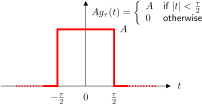
\includegraphics[width=8cm]{cuadrada}
  \end{center}
  \else
  \HCode{
    <div style="text-align:center;">
    <img height="250" src="data/cuadrada.png" />
    </div>
  }
  \fi
  Determine its Fuorier spectrum.
%\item [] Antes de aplicar la Ecuaci\'on \ref{eq:Fw} que calcula la
%  transformada (directa) de Fourier, vamos a realizar un cambio de
%  notaci\'on en ella que exprese la frecuencia en Hercios en lugar de
%  radianes/segundo. As\'{\i}, dicha ecuaci\'on quedar\'{\i}a como
%  \begin{equation}
%    F(2\pi f) = \int_{-\infty}^{-\infty} f(t)e^{(-2\pi fjt)}dt.
%    \label{eq:Fw2}
%  \end{equation}
%  Substituyendo para el caso del ejemplo, llegamos a que
%  $$
%  \begin{array}{ll}
%    F(2\pi f) & = \displaystyle\int_0^X Ae^{(-2\pi fjt)}dt \\
%    & = \displaystyle\frac{-A}{2\pi jf}e^{(-2\pi
%      fjt)}\displaystyle|_0^X\\
%    & = \displaystyle\frac{-A}{2\pi jf}(e^{(-2\pi
%      fjt)}-1)\\
%    & = \displaystyle\frac{A}{2\pi jf}[e^{(\pi
%      fjt)}-e^{(-\pi fjt)}]e^{(-\pi fjt)}\\
%    & = \displaystyle\frac{A}{\pi f}\sin(X\pi f)e^{(-jX\pi f)}\\
%    & = AX\displaystyle\frac{\sin(X\pi f)}{X\pi f}e^{(-jX\pi f)}\\
%    & = AX\mathrm{sinc}(X\pi f)e^{(-jX\pi f)},
%  \end{array}
%  $$
%  que como puede verse, se trata de un espectro complejo.

\item[] Applying the \ref{eq:Ft} Equation we have that
  \begin{equation*}
    F(\omega) = \displaystyle\int_{-\frac{\tau}{2}}^{\frac{\tau}{2}}
    Ae^{-j\omega t}dt = \displaystyle\frac{A}{j\omega}e^{-j\omega
      t}\displaystyle|_{-\frac{\tau}{2}}^{\frac{\tau}{2}} =
    \displaystyle\frac{A}{j\omega}(e^{j\omega\frac{\tau}{2}}-e^{-j\omega\frac{\tau}{2}})
  \end{equation*}
  Considering that $e^{jx}-e^{-jx}=2j\sin(x)$.
  \begin{equation*}
   F(\omega)=
   A\tau\displaystyle\frac{\sin(\omega\frac{\tau}{2})}{\omega\frac{\tau}{2}}
   = A\tau\mathrm{Sinc}(\omega\frac{\tau}{2}).
  \end{equation*}
  
\item [] The function
  \begin{equation*}
    \mathrm{Sinc}(x) = \frac{\sin(x)}{x}
  \end{equation*}
  it is called \emph{sampling function} and it is very important in
  Signal Communication Theory because, as we will see, it is the
  function used by Digital / Analogic converters to pass the digitized
  signal from pulse modulation to its original continuous
  representation~\cite{Lathi}.
  
\item [] Note that $F(\omega)$ is a real function and therefore can be represented graphically by a single curve\footnote{If it were a complex function, we would represent the spectrum module and its phase.}
  %$$
  %|F(2\pi f)| = AX|\mathrm{sinc}(X\pi f)||e^{(-jX\pi f)}| = AX|\mathrm{sinc}(X\pi f)|
  %$$
  %que representado gr\'aficamente se corresponde a
  
\end{itemize}

\ifx\HCode\Undfef
\begin{center}
  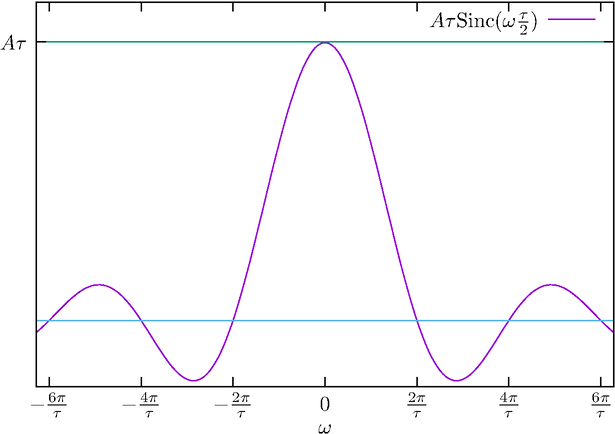
\includegraphics[width=0.9\textwidth]{funcion_muestreo_small}
\end{center}
\else
\HCode{
  <div style="text-align:center;">
  <img height="350" src="data/funcion_muestreo_small.png" />
  </div>
}
\fi

\noindent Notice that if if $\tau\rightarrow \infty$ then the spectrum
tends to become an impulse at $\omega=0$ and if $\tau\rightarrow 0$
then the spectrum tends to become a constant function.

\section{The Dirac (unit impulse) function}
\begin{itemize}
\item The unit impulse function \cite{Lathi} plays a determining role
  in the theory of signal communication and in particular in the
  sampling theorem. It is defined as:
  \ifx\HCode\Undfef
  \begin{center}
    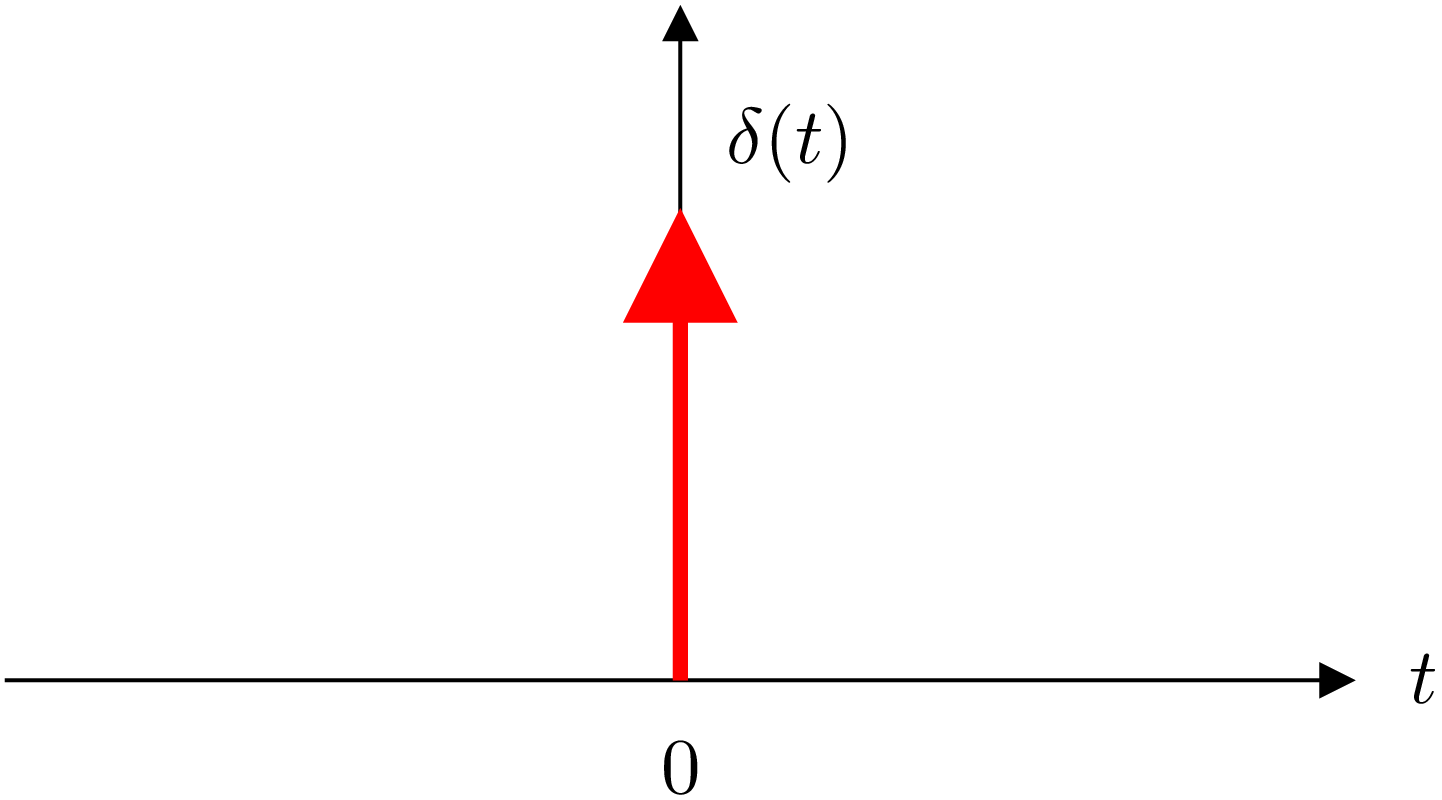
\includegraphics[width=8cm]{delta}
    %\texfigure{!}{!}{delta}
  \end{center}
  \else
  \HCode{
    <div style="text-align:center;">
    <img height="250" src="data/delta.png" />
    </div>
  }
  \fi
  and it fulfills that
  \begin{equation}
    \left\{
      \begin{array}{ll}
        \displaystyle\int_{-\infty}^\infty\delta(t)dt=1 & \text{si $t=0$}\\
        0 & \text{resto,}
      \end{array}
    \right.
    \tag{delta\_1}
    \label{eq:delta_1}
  \end{equation}
  that is, although it is an infinitely narrow pulse, it has an area
  of $1$ because it has infinite amplitude. For the same reason we have,
  by definition, that (\ref{eq:delta_2})
  % \begin{equation}
  %   f(t)\delta(t) = f(0)
  %   \label{eq:delta}
  % \end{equation}
  % y que
  \begin{equation}
    \int_{-\infty}^\infty\delta(t)f(t)dt =
    f(0)\int_{-\infty}^\infty\delta(t)dt = f(0),
    \tag{delta\_2}
    \label{eq:delta_2}
  \end{equation}
  and in the same way, that
  \begin{equation*}
    \int_{-\infty}^\infty\delta(t-t_0)f(t)dt = f(t_0).
  \end{equation*}
\item By virtue of these definitions we could say that the unit
  impulse function is able to calculate the value of a function at the
  point where it is defined (the delta).
\end{itemize}

\subsection{Generating the Dirac function}
% {{{ 

\begin{itemize}
\item The unit impulse function is a function physically impossible to
  generate and that is obtained in the limit of other functions:
  \begin{enumerate}
  \item From a rectangular function:
    \ifx\HCode\Undfef
    \begin{center}
      %\texfigure{!}{!}{limite}
      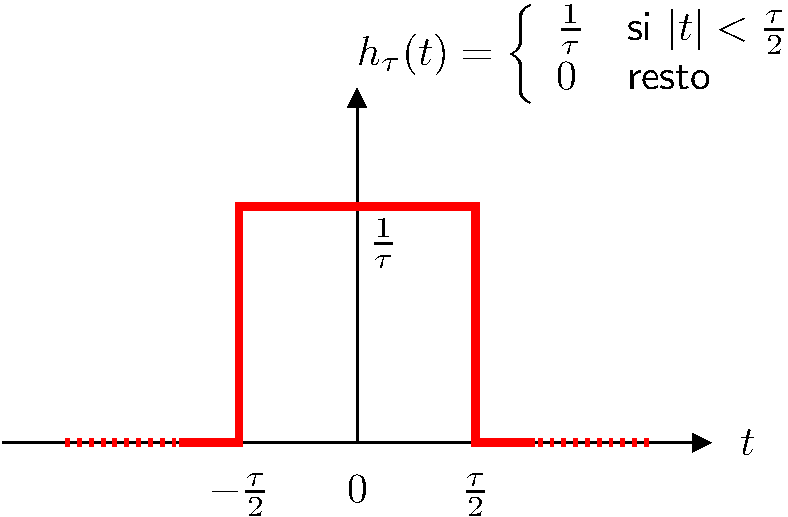
\includegraphics[width=8cm]{limite}
    \end{center}
    \else
    \HCode{
      <div style="text-align:center;">
      <img height="250" src="data/limite.png" />
    </div>
    }
    \fi
    taking
    $$
    \lim_{\tau\rightarrow0}h_\tau(t) = \delta(t).
    $$
  \item From the sampling function:
    \begin{equation}
      \delta(t) =
      \lim_{\tau\rightarrow\infty}\frac{\tau}{\pi}\mathrm{Sinc}(\tau
      t).  \tag{delta\_muestreo}
      \label{eq:delta_muestreo}
    \end{equation}
    %N\'otese que el area que hay entre la curva de la funci\'on
    %muestreo y el eje del tiempo $t$ es $2\pi$.  Note that when
    $\tau$ increases, the sampling function is compacted at $t=0$.
  \end{enumerate}
\end{itemize}

\section{Fourier transform of the unit impulse function}
\begin{itemize}
\item [] The Fourier transform of the unit impulse function is
  $1$. That is to say (\ref{eq:TFdelta}),
  \begin{equation}
    {\cal{F}}[\delta(t)]=1.
    \tag{FT$\delta$}
    \label{eq:TFdelta}
  \end{equation}
  graphically:
  \ifx\HCode\Undfef
  \begin{center}
    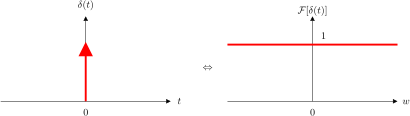
\includegraphics[width=0.9\textwidth]{delta_1}
  \end{center}
  \else
  \HCode{
    <div style="text-align:center;">
    <img height="250" src="data/delta_1.png" />
    </div>
  }
  \fi
\end{itemize}
\subsection*{Proof}
By de fi nition of the Fourier transform (see Equation \ref{eq:Ft}) one has to:
\begin{equation*}
  \begin{array}{rcl}
    {\cal F}[\delta(t)] & = & \displaystyle\int_{-\infty}^\infty\delta(t)e^{-j\omega t}dt\\\\
    \multicolumn{3}{l}{\text{(Aplicando \ref{eq:delta_2} y \ref{eq:delta_1})}}\\\\
    & = & \underbrace{e^{-j\omega_0}}_{1}\underbrace{\displaystyle\int_{-\infty}^\infty\delta(t)dt}_{1} = 1.
  \end{array}
\end{equation*}

\section{Fourier transform of the constant function}
\begin{itemize}
\item [] The Fourier transform of the constant function 1 is the
  impulse function, multiplied by $2\pi$. That is to say,
  \begin{equation}
    {\cal{F}}[1] = \int_{-\infty}^\infty e^{-j\omega t}dt = 2\pi\delta(\omega).
    \tag{Ftcf}
    \label{eq:TFfc}
  \end{equation}
  Graphically:
  \ifx\HCode\Undfef
  \begin{center}
    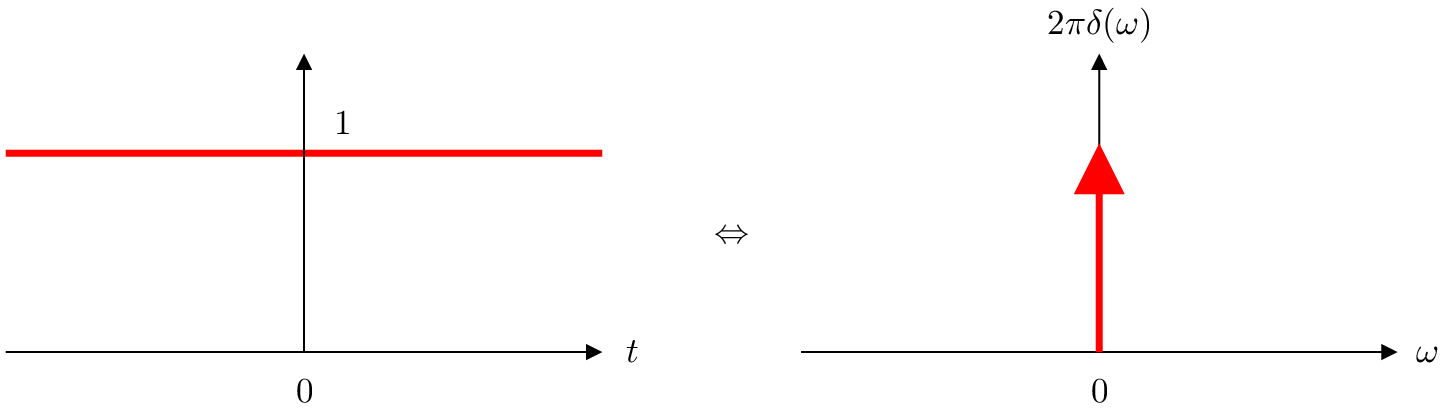
\includegraphics[width=0.9\textwidth]{1_delta}
  \end{center}
  \else
  \HCode{
    <div style="text-align:center;">
    <img height="250" src="data/1_delta.png" />
    </div>
  }
  \fi
\end{itemize}

\subsection*{Proof}
\begin{itemize}
\item As we know, the Fourier transform of a rectangular function is
  the Sinc function (see Section \ref{sec:funcion_muestreo}), that is,
  \begin{equation*}
    {\cal F}[g_\tau(t)] = \tau\mathrm{Sinc}(\frac{\tau}{2}\omega).
  \end{equation*}
\item On the other hand, the rectangular function tends to become a
  constant function when $\tau\rightarrow\infty$, i.e.
  \begin{equation*}
    \lim_{\tau\rightarrow\infty} g_\tau(t) = 1.
  \end{equation*}
\item Consequently, the Fourier transform of the constant function $1$ is the Fourier transform of a rectangular function $g_\tau(t)$, when $\tau\rightarrow\infty$, i.e.
  \begin{equation*}
    {\cal F}[1] = \displaystyle\lim_{\tau\rightarrow\infty} \tau\mathrm{Sinc}(\frac{\tau}{2}\omega)
  \end{equation*}
  Multiplying and dividing by $2\pi$.
  \begin{equation*}
    {\cal F}[1] = \displaystyle2\pi\lim_{\tau\rightarrow\infty}
    \frac{\tau}{2\pi}\text{Sinc}(\frac{\tau}{2}\omega)
  \end{equation*}
  Applying Eq. \ref{eq:delta_muestreo} for $\frac{\tau}{2}$.
  \begin{equation*}
    {\cal F}[1] =2\pi\delta(\omega).
  \end{equation*}
  
\end{itemize}

\section{Transformada de Fourier de la funci\'on exponencial compleja}
%\section{Fourier transform of the complex exponential function}
\begin{itemize}
\item The Fourier transform of the complex exponential function of
  frequency $\omega_0$ is a unit impulse of energy $2\pi$ in $\omega_0$,
  \begin{equation}
    {\cal F }[e^{j\omega_0t}] = 2\pi\delta(\omega-\omega_0).
    \tag{FTCE}
    \label{eq:FTCE}
  \end{equation}
\item Graphically:
  \ifx\HCode\Undfef
  \begin{center}
    %\texfigure{0.6\textwidth}{!}{TFexpo}
    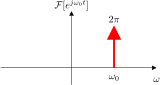
\includegraphics[width=0.6\textwidth]{TFexpo}
  \end{center}
  \else
  \HCode{
    <div style="text-align:center;">
    <img height="200" src="data/TFexpo.png" />
    </div>
  }
  \fi
\end{itemize}

\subsection*{Proof}
\noindent By definition,
\begin{equation*}
  {\cal F}[e^{j\omega_0t}] = \int_{-\infty}^\infty e^{j\omega_0t}e^{-j\omega t} dt =
  \int_{-\infty}^\infty e^{-j(\omega-\omega_o)t}dt.
\end{equation*}
Taking into cosideration Eq. \ref{eq:TFfc} and substituting 
$\omega=\omega-\omega_0$ we get that
\begin{equation*}
  {\cal F}[e^{j\omega_0t}] = 2\pi\delta(\omega-\omega_0).
\end{equation*}

\section{Fourier transform of the sine function}
\begin{itemize}
\item The Fourier transform of the frequency sine function $\omega_0$ are two
  energy pulses $j\pi$, one positive in $-\omega_0$ and another negative in $\omega_0$,
  i.e.
  \begin{equation}
    {\cal F}[\sin(\omega_0t)] = j\pi\big(\delta(\omega+\omega_0)-\delta(\omega-\omega_0)\big).
    \tag{FTsin}
    \label{eq:TFsen}
  \end{equation}
  Graphically:
  \ifx\HCode\Undfef
  \begin{center}
    %\texfigure{0.9\textwidth}{!}{TFseno}
    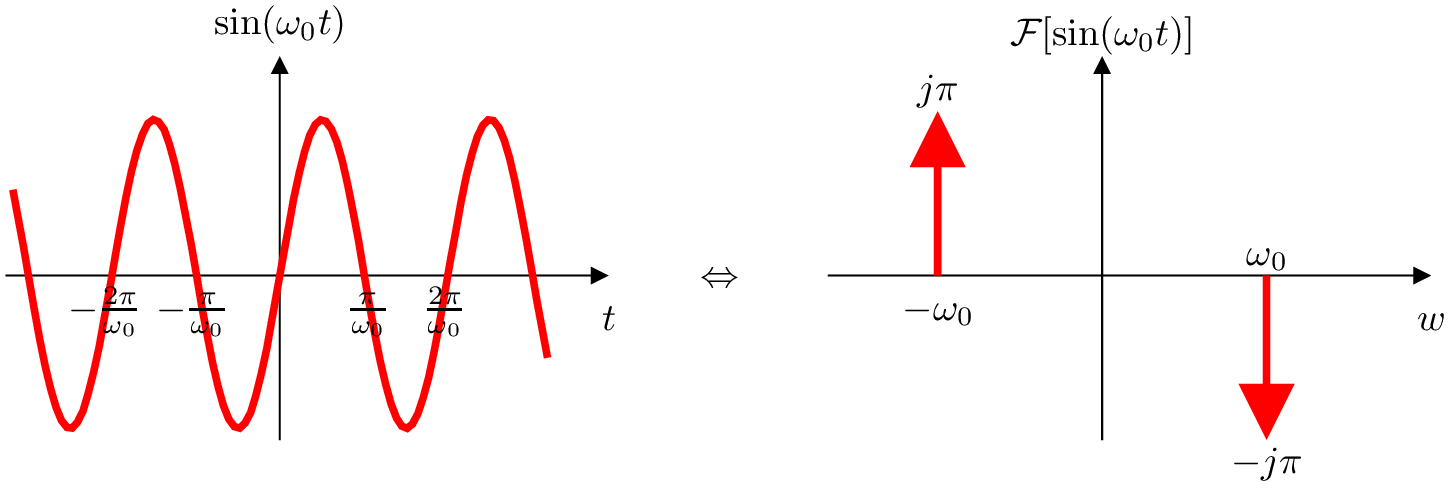
\includegraphics[width=0.9\textwidth]{TFseno}
  \end{center}
  \else
  \HCode{
    <div style="text-align:center;">
    <img height="200" src="data/TFseno.png" />
    </div>
  }
  \fi
\end{itemize}

\subsection*{Proof}
\noindent As we know,
\begin{equation*}
  \sin(\omega_0t) = \frac{\displaystyle e^{j\omega_0t}-e^{-j\omega_0t}}{\displaystyle 2j}.
\end{equation*}
Therefore (see \ref{eq:FTCE}),
\begin{equation*}
  \begin{array}{rl}
    {\cal F}[\sin(\omega_0t)] & = \displaystyle\frac{1}{2j}({\cal
      F}[e^{j\omega_0t}]-{\cal F}[e^{-j\omega_0t}])\\\\
    & = \displaystyle\frac{1}{2j}\big(2\pi\delta(\omega-\omega_0)-2\pi\delta(\omega+\omega_0)\big)\\\\
    & = j\pi\big(\delta(\omega+\omega_0)-\delta(\omega-\omega_0)\big).
  \end{array}
\end{equation*}

\section{Fourier transform of the cosine function}
\begin{itemize}
\item The Fourier transform of the cosine function of frequency $\omega_0$
  are two positive pulses of energy $j\pi$, one in $-\omega_0$ and another
  in $\omega_0$, i.e.
  \begin{equation}
    {\cal F}[\cos(\omega_0t)] = j\pi\big(\delta(\omega+\omega_0)+\delta(\omega-\omega_0)\big).
    \tag{FTCos}
    \label{eq:FtCos}
  \end{equation}
  Graphically:
  \ifx\HCode\Undfef
  \begin{center}
    %\    texfigure{0.9\textwidth}{!}{TFcoseno}
    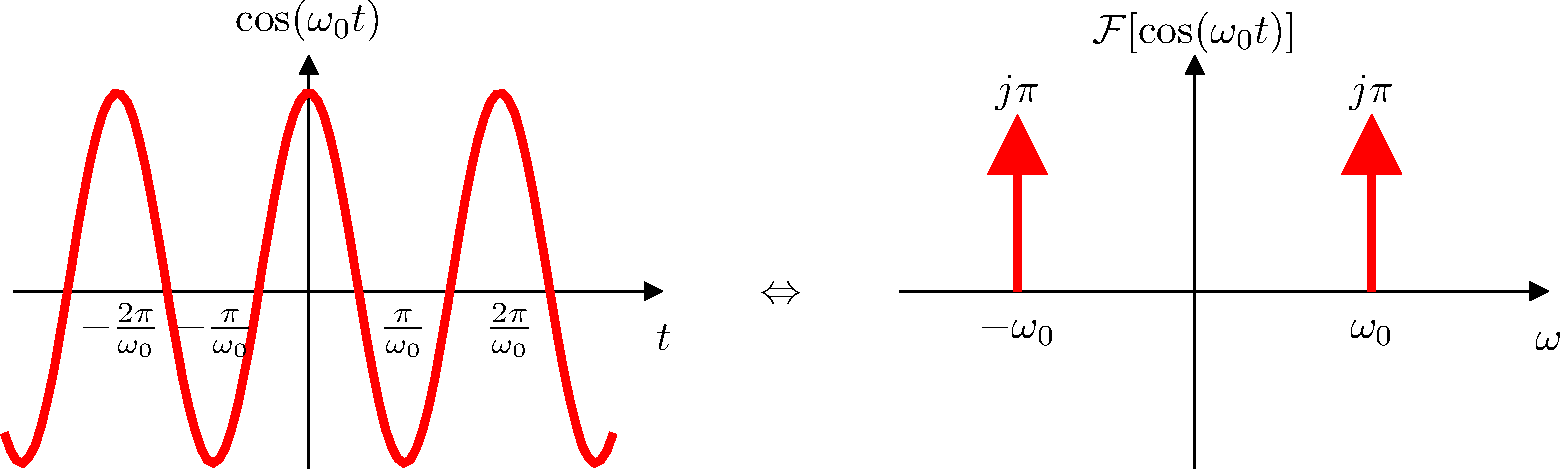
\includegraphics[width=0.9\textwidth]{TFcoseno}
  \end{center}
  \else
  \HCode{
    <div style="text-align:center;">
    <img height="200" src="data/TFcoseno.png" />
    </div>
  }
  \fi
\end{itemize}

\subsection*{Proof}
\noindent We know that,
\begin{equation}
  \cos(\omega_0t) = \frac{\displaystyle e^{j\omega_0t}+e^{-j\omega_0t}}{\displaystyle 2j}.
\end{equation}
Therefore (see \ref{eq:FTCE}),
\begin{equation*}
  \begin{array}{rl}
    {\cal F}[\cos(\omega_0t)] & = \displaystyle\frac{1}{2j}({\cal
      F}[e^{j\omega_0t}]+{\cal F}[e^{-j\omega_0t}])\\\\
    & = \displaystyle\frac{1}{2j}\big(2\pi\delta(\omega-\omega_0)+2\pi\delta(\omega+\omega_0)\big)\\\\
    & = j\pi\big(\delta(\omega+\omega_0)+\delta(\omega-\omega_0)\big).
  \end{array}
\end{equation*}

\section{Fourier transform of a periodic function}
\begin{itemize}
\item We can express any periodic function $f(t)$ by its exponential
  Fourier series (see Equation \ref{eq:Fes})
  \begin{displaymath}
    \begin{array}{rl}
      {\cal F}[f(t)] & = {\cal F}[\displaystyle\sum_{n=-\infty}^\infty F_n
      e^{jn\omega_ot}]\\\\
      & = \displaystyle\sum_{n=-\infty}^\infty F_n{\cal F}[e^{jn\omega_ot}].
    \end{array}
  \end{displaymath}
  Using the Expression \ref{eq:FTCE}, we get that
  \begin{equation}
    {\cal F}[f(t)] = 2\pi\sum_{n=-\infty}^\infty F_n\delta(\omega-n\omega_0).
    \tag{Ftpf}
    \label{eq:TFfp}
  \end{equation}

\item This relationship is very important because it establishes that
  the spectral density function (the Fourier transform) of a periodic
  signal is composed of pulses located at harmonic frequencies
  (frequencies multiples of the fundamental frequency $\omega_0$) of said
  signal, being the energy of each impulse $2\pi$ multiplied by the
  value of the corresponding coefficient of the exponential Fourier
  series.

\item Graphically, for the case of the rectangular function:
\end{itemize}
\ifx\HCode\Undfef
\begin{center}
  %\texfigure{\textwidth}{!}{TFfuncion_periodica}
  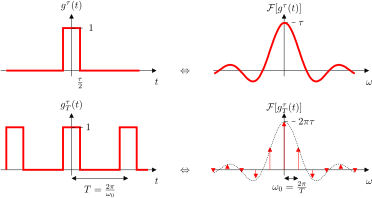
\includegraphics[width=\textwidth]{TFfuncion_periodica}
\end{center}
\else
\HCode{
  <div style="text-align:center;">
  <img height="500" src="data/TFfuncion_periodica.png" />
  </div>
}
\fi

\section{Fourier transform of an impulse train function}
\begin{itemize}
\item The train function of equidistant unitary pulses is very
  important in sampling theory because it mathematically represents
  the signal sampling process.
\item Let the unit impulse train function
  \begin{equation}
    \delta_T(t) = \sum_{n=-\infty}^{\infty}\delta(t-nT).
    \tag{$\delta_T$}
    \label{eq:delta_T}
  \end{equation}
  So, its Fourier transform is anoter pulee train
  (\ref{eq:TF_delta_T})
  \begin{equation}
    {\cal F}[\delta_T(t)] = \omega_0\sum_{n=-\infty}^{\infty}\delta(\omega-n\omega_0)
    = \omega_0\delta_{\omega_0}(\omega).
    \tag{${\cal F}[\delta_T(t)]$}
    \label{eq:TF_delta_T}
  \end{equation}
\end{itemize}
\ifx\HCode\Undfef
\begin{center}
  %\texfigure{\textwidth}{!}{TFtren_de_impulsos}
  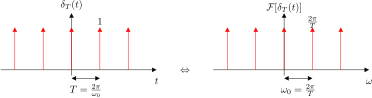
\includegraphics[width=\textwidth]{TFtren_de_impulsos}
\end{center}
\else
\HCode{
  <div style="text-align:center;">
  <img height="500" src="data/TFtren_de_impulsos.png" />
  </div>
}
\fi
\begin{itemize}
\item Note that as $T$ increases the spectrum becomes denser and its
  amplitude decreases.
\end{itemize}

\subsection*{Proof}
\begin{itemize}
\item [] The exponential Fourier series of $\delta_T(t)$ is
  \begin{equation*}
    \delta_T(t)=\sum_{n=-\infty}^{\infty}F_ne^{jn\omega_0t}
  \end{equation*}
  where
  \begin{equation*}
    \omega_0 = \frac{2\pi}{T}
  \end{equation*}
  and
  \begin{equation*}
    F_n = \frac{1}{T}\int_{-\frac{T}{2}}^{\frac{T}{2}}\delta_T(t)e^{-jn\omega_0t}dt.
  \end{equation*}
  Function $\delta_T(t)$ in the interval
  $(-\frac{T}{2},\frac{T}{2})$ simply is $\delta(t)$. Therefore
  \begin{equation*}
  F_n = \frac{1}{T}\int_{-\frac{T}{2}}^{\frac{T}{2}}\delta(t)e^{-jn\omega_0t}dt.
  \end{equation*}
  Because of the way in which the unit impulse function is defined, it
  is necessary to
  \begin{equation*}
    \frac{1}{T}\int_{-\frac{T}{2}}^{\frac{T}{2}}\delta(t)e^{-jn\omega_0t}dt =
    \frac{1}{T}\int_{-\infty}^{\infty}\delta(t)e^{-jn\omega_0t}dt.
  \end{equation*}
  Applying now the de fi nition of the function $\delta(t)$
  (Expression \ref{eq:delta_2}) one has
  \begin{equation*}
  F_n = \frac{e^{jn\omega_00}}{T}\int_{-\infty}^{\infty}\delta(t)dt = \frac{1}{T}
  \end{equation*}
  %y teniendo en cuenta que
  %$$
  %\int_{-\frac{T}{2}}^{\frac{T}{2}}e^{-jn\omega_0t}dt = 1
  %$$
  %llegamos a que
  %$$
  %F_n = \frac{1}{T}.
  %$$
  and therefore, that
  \begin{equation*}
  \delta_T(t) = \frac{1}{T}\sum_{n=-\infty}^{\infty}e^{jn\omega_0t}.
  \end{equation*}
  To find its Fourier transform we resort to the Equation
  \ref{eq:TFfp}. So we get to that
  \begin{equation*}
    \begin{array}{rl}
      {\cal F}[\delta_T(t)] & =
      2\pi\displaystyle\sum_{n=-\infty}^\infty\frac{1}{T}\delta(\omega-n\omega_0)\\\\
      & =
      \displaystyle\frac{2\pi}{T}\sum_{n=-\infty}^\infty\delta(\omega-n\omega_0)\\\\
      & = \omega_0\displaystyle\sum_{n=-\infty}^\infty\delta(\omega-n\omega_0)\\\\
      & = \omega_0\delta_{\omega_0}(\omega).
    \end{array}
  \end{equation*}
\end{itemize}

\section{Fourier transform of a time-shifted signal}
\begin{itemize}
\item [] If
  \begin{equation*}
  {\cal F}[f(t)] = F(\omega)
  \end{equation*}
  then
  \begin{equation}
    {\cal F}[f(t-t_0)] = F(\omega)e^{-j\omega t_0}.
    \tag{${\cal F}[f(t-t_0)]$}
    \label{eq:TFfdt}
  \end{equation}
  That is, moving a function over time is equivalent to multiplying in
  the domain of the frequency by the complex exponential function.
\end{itemize}

\subsection*{Proof}
\noindent By definition of Fourier transform we have that
$$
{\cal F}[f(t-t_0)] = \int_{-\infty}^\infty f(t-t_0)e^{-j\omega t}dt.
$$
Be $x=t-t_0$. Then
$$
\begin{array}{rl}
  {\cal F}[f(t-t_0)] & = \displaystyle\int_{-\infty}^\infty
  f(x)e^{-j\omega(x+t_0)}dx\\\\
  & = \displaystyle\int_{-\infty}^\infty f(x)e^{-j\omega x}dx\cdot e^{-j\omega t_0}\\\\
  & = F(\omega)e^{-j\omega t_0}.
\end{array}
$$

%}}}

\section{Inverse Fourier transform of a time-shifted function}

\begin{itemize}
\item [] If
  \begin{equation*}
    {\cal F}[f(t)] = F(\omega)
  \end{equation*}
  then
  \begin{equation}
    F(\omega-\omega_0) = {\cal F}[f(t)e^{j\omega_0t}].
    \tag{$F(\omega-\omega_0)$}
    \label{eq:TFifdf}
  \end{equation}
  That is, moving the spectrum of a function is equivalent to
  multiplying that function in the time domain by a complex
  exponential.
\end{itemize}

\subsection*{Proof}
\noindent By definition of Fourier transform one has to
\begin{equation*}
  \begin{array}{rl}
    {\cal F}[f(t)e^{j\omega_0t}] & = \displaystyle\int_{-\infty}^\infty
    [f(t)e^{j\omega_0t}]e^{-j\omega t}dt\\\\
    & = \displaystyle\int_{-\infty}^\infty
    f(t)e^{-j(\omega-\omega_0)t}dt\\\\
    \multicolumn{2}{l}{\text{(Por definici\'on de transformada de Fourier
        para $\omega=\omega-\omega_0$)}}\\\\
    & = F(\omega-\omega_0).
  \end{array}
\end{equation*}

\section{Functions convolution}
\begin{itemize}
\item Be $f_1(t)$ and $f_2(t)$ two functions. Their convolution
  $f_1(t)*f_2(t)$ is defined as~\cite{Gonzalez}
  \begin{equation}
    f_1(t)*f_2(t)=\int_{-\infty}^\infty f_1(\tau)f_2(t-\tau)d\tau.
    \tag{$f_1(t)*f_2(t)$}% \tag{Conv-func}
    \label{eq:convolucion}
  \end{equation}
\end{itemize}

\subsection*{Example}
\begin{center}
  %\texfigure{!}{7cm}{ejemplo_convolucion}
  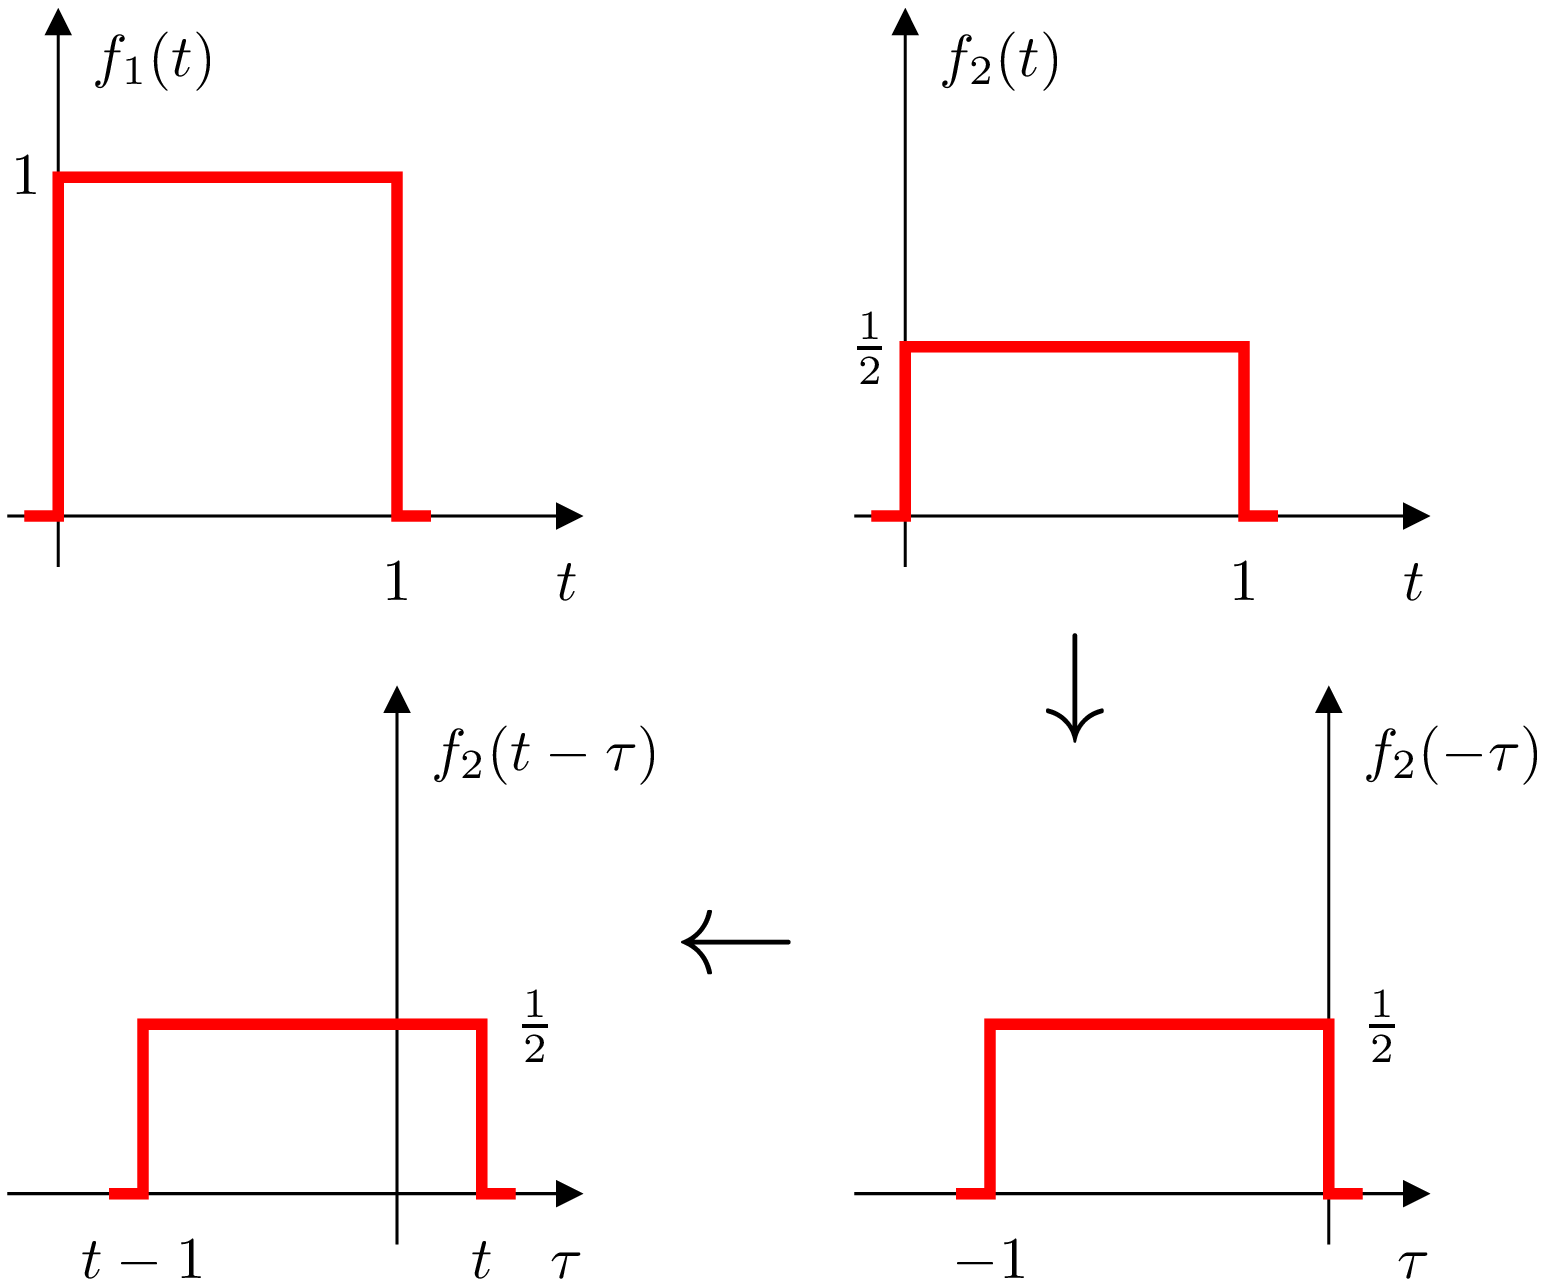
\includegraphics[height=7cm]{ejemplo_convolucion}
\end{center}
\begin{itemize}
\item The convolution of two functions $f_1(t)$ and $f_2(t)$ is
  calculated for the different values of $t$ that shifts to
  $f_2(t-\tau)$ in $t$ (seconds) and calculating the area of
  superposition of the functions. Thus:
  \begin{enumerate}
    \item If $t<0$ we get that:
      \begin{center}
        %\texfigure{!}{!}{caso1}
        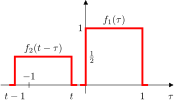
\includegraphics[width=8cm]{caso1}
      \end{center}
      and as can be seen, there is no overlap, that is,
      $f_1(\tau)f_2(t-\tau)=0$.
    \item If $t=0$:
      \begin{center}
        %\texfigure{!}{!}{caso2}
        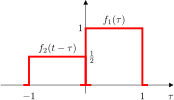
\includegraphics[width=8cm]{caso2}
      \end{center}
      overlapping begins to exist.
    \item If $t=1/2$:
      \begin{center}
        %\texfigure{!}{!}{caso3}
        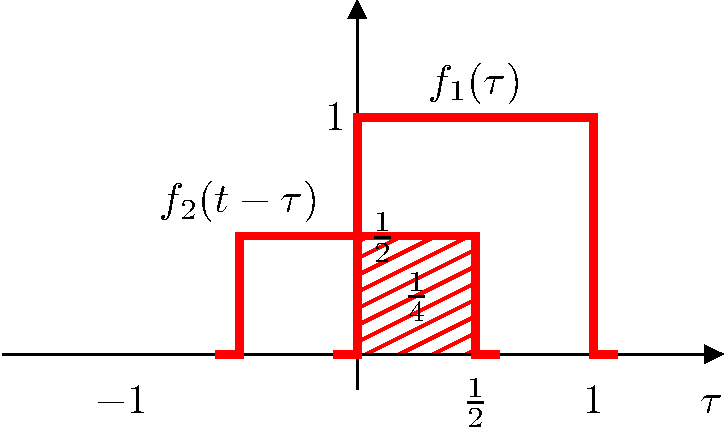
\includegraphics[width=8cm]{caso3}
      \end{center}
      the overlap area is 1/4.
    \item If $t=1$:
      \begin{center}
        %\texfigure{!}{!}{caso4}
        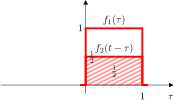
\includegraphics[width=8cm]{caso4}
      \end{center}
      the area is 1/2.
    \item If $t=3/4$:
      \begin{center}
        %\texfigure{!}{!}{caso5}
        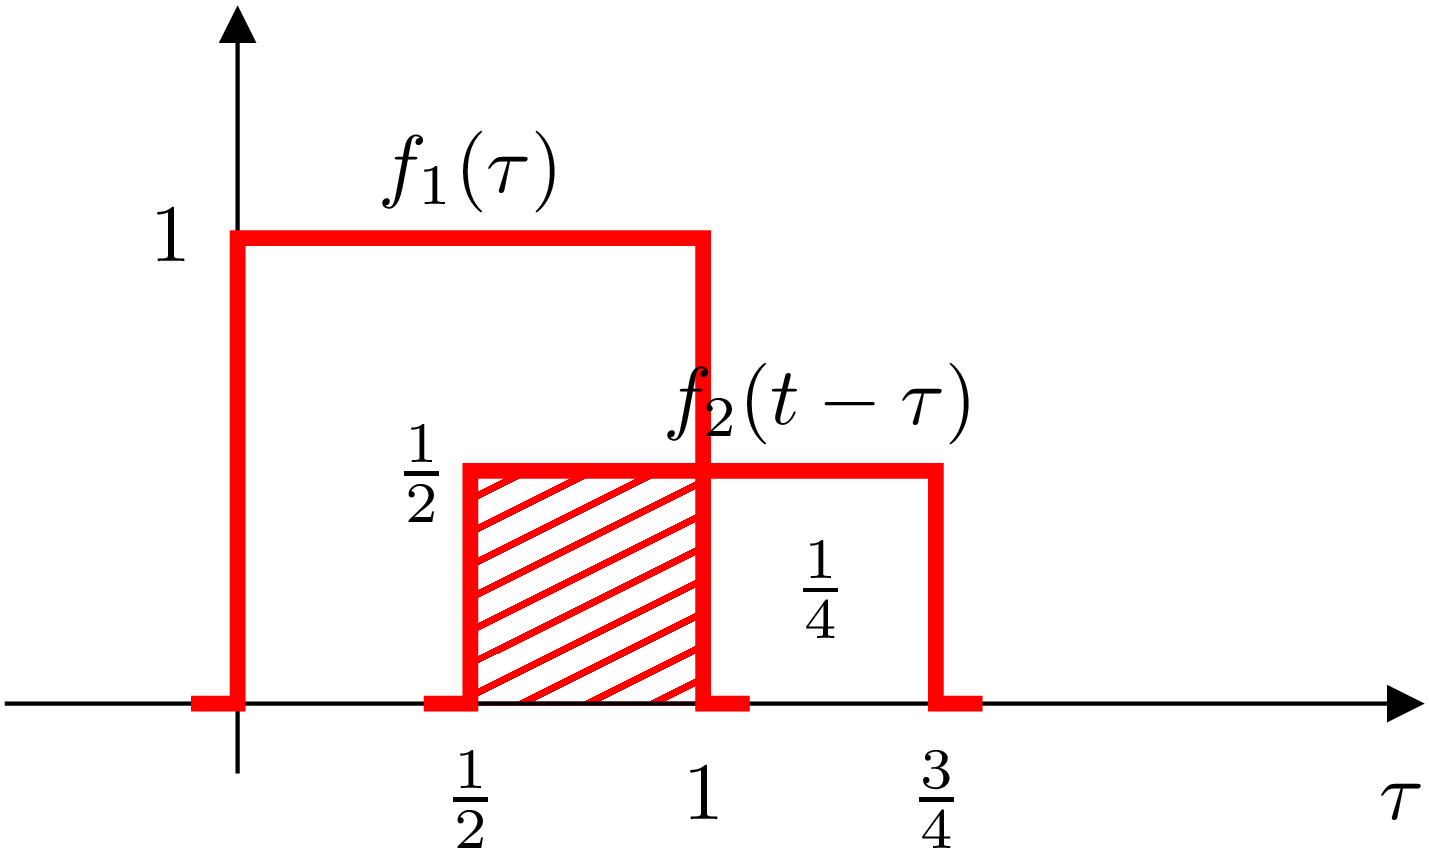
\includegraphics[width=8cm]{caso5}
      \end{center}
      the overlap area is 1/4.
    \item If $t=2$:
      \begin{center}
        %\texfigure{!}{!}{caso6}
        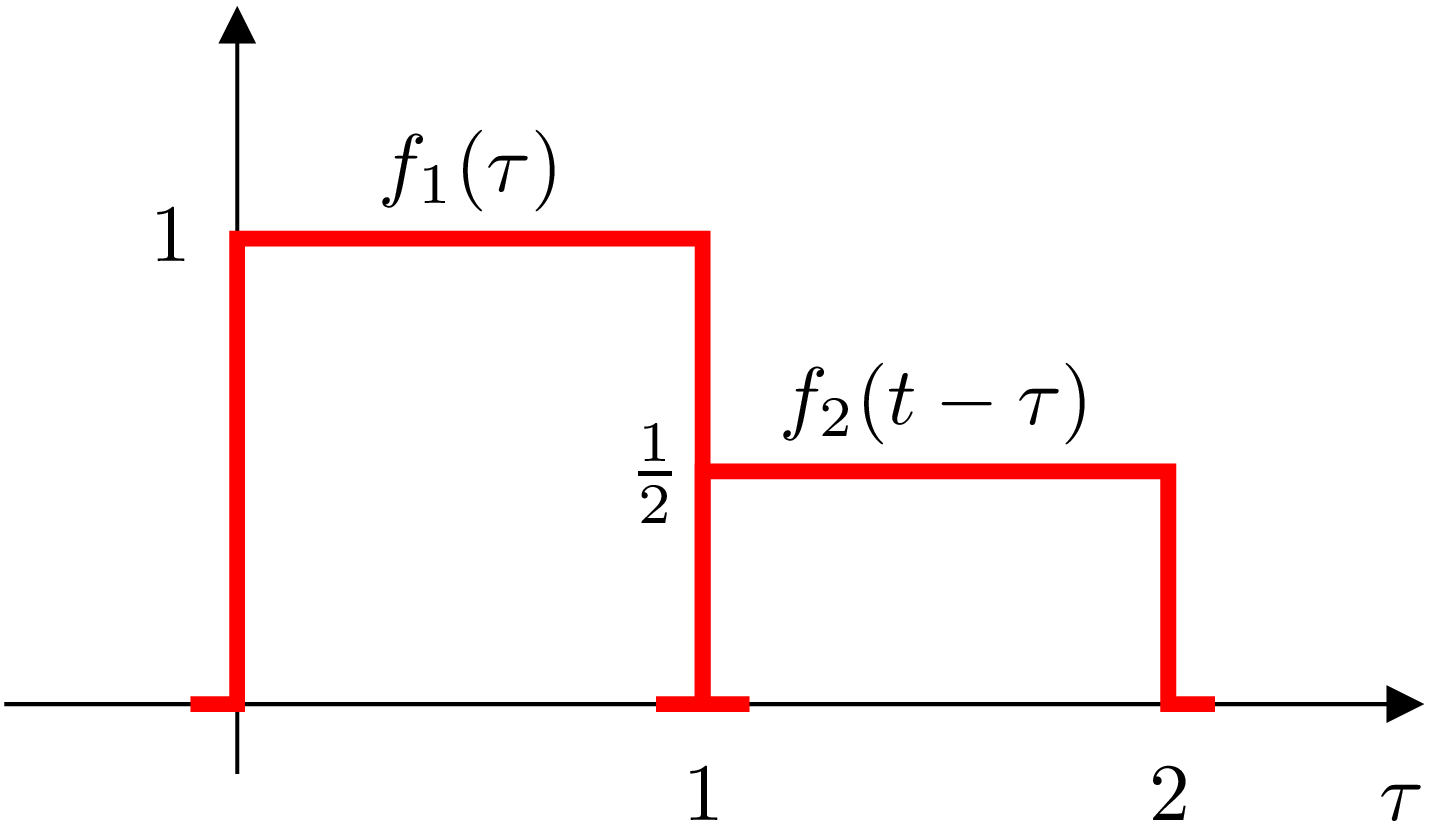
\includegraphics[width=8cm]{caso6}
      \end{center}
      the overlap area is again 0.
  \end{enumerate}
\item Therefore:
  \begin{center}
    %\texfigure{!}{!}{final}
    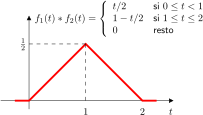
\includegraphics[width=8cm]{final}
  \end{center}
\end{itemize}

\section{The time-domain convolution theorem}
\begin{itemize}
\item It establishes that the convolution of two functions $f_1(t)$ and
  $f_2(t)$ in the time domain is equivalent to multiplying their spectra
  $F_1(\omega)$ and $F_2(\omega)$, that is,
%y luego realizar la transformada inversa de Fourier, es decir,
\begin{equation}
  f_1(t)*f_2(t) = {\cal F}^{-1}[F_1(\omega)F_2(\omega)].
  \tag{ConvT}
  \label{eq:teorema_convolucion_tiempo}
\end{equation}
\end{itemize}

\subsection*{Proof}
\noindent By definition of the Fourier transform and the convolution
operation one has to
\begin{equation*}
  \begin{array}{rl}
    {\cal F}[f_1(t)*f_2(t)] & = \displaystyle\int_{-\infty}^\infty
    \Big[\int_{-\infty}^\infty
      f_1(\tau)f_2(t-\tau)d\tau\Big]e^{-j\omega t}dt\\\\
    & = \displaystyle\int_{-\infty}^\infty
    f_1(\tau)\Big[\underbrace{\int_{-\infty}^\infty f_2(t-\tau)e^{-j\omega t}dt}_{F_2(\omega)e^{-j\omega\tau}}\Big]d\tau.
  \end{array}
\end{equation*}
Note that
\begin{equation*}
  \int_{-\infty}^\infty f_2(t-\tau)e^{-j\omega t}dt = {\cal{F}}\{f_2(t-\tau)\}
\end{equation*}
and appliying the Expression \ref{eq:TFfdt} we get that
\begin{equation*}
  \int_{-\infty}^\infty f_2(t-\tau)e^{-j\omega t}dt = F_2(\omega)e^{-j\omega\tau}.
\end{equation*}
Therefore,
\begin{equation*}
  \begin{array}{rl}
    {\cal F}[f_1(t)*f_2(t)] & = \displaystyle\int_{-\infty}^\infty
    f_1(\tau)F_2(\omega)e^{-j\omega\tau}d\tau \\\\
    & = F_2(\omega)\displaystyle\int_{-\infty}^\infty f_1(\tau)e^{-j\omega\tau}d\tau\\\\
    & = F_1(\omega)F_2(\omega).
  \end{array}
\end{equation*}

\section{The frequency-domain convolution theorem}
\begin{itemize}
\item It establishes that the multiplication of two functions $f_1(t)$
  and $f_2(t)$ in the time domain is equivalent (except for a scale
  factor) when convolving its $F_1(\omega)$ and $F_2(\omega)$ spectra,
  i.e.
  % y luego realizar la transformada inversa de Fourier, es decir,
  \begin{equation}
    f_1(t)f_2(t) = {\cal
      F}^{-1}\Big[\frac{1}{2\pi}\big(F_1(\omega)*F_2(\omega)\big)\Big].
    \tag{ConvF}
    \label{eq:teorema_convolucion_frecuencia}
  \end{equation}
\end{itemize}

\subsection*{Proof}
By definition of the inverse Fourier transform (Eq. \ref{eq:iFt})
\begin{equation*}
  {\cal F}^{-1}\Big[\displaystyle\frac{1}{2\pi}\big(F_1(\omega)*F_2(\omega)\big)\Big] =
  \displaystyle\frac{1}{2\pi}\displaystyle\int_{-\infty}^\infty
  \Big[\frac{1}{2\pi}\big(F_1(\omega)*F_2(\omega)\big)\Big]e^{j\omega t}d\omega
\end{equation*}

By definition of convolution (Eq. \ref{eq:convolucion})
\begin{equation*}
=
  \displaystyle\frac{1}{2\pi}\displaystyle\int_{-\infty}^\infty
  \Big[\frac{1}{2\pi}\big(\displaystyle\int_{-\infty}^\infty
    F_1(\tau)F_2(\omega-\tau)d\tau\big)\Big]e^{j\omega t}d\omega
\end{equation*}

rearranging
\begin{equation*}
=
  \displaystyle\frac{1}{2\pi}\displaystyle\int_{-\infty}^\infty
  F_1(\tau)\Big[\frac{1}{2\pi}\displaystyle\int_{-\infty}^\infty
  F_2(\omega-\tau)e^{j\omega t}d\omega\Big]d\tau.
\end{equation*}

If we use now the Eq. \ref{eq:TFifdf} and we apply the inverse Fourier
transform we get to that
\begin{equation*}
  \frac{1}{2\pi}\int_{-\infty}^\infty F_2(\omega-\tau)e^{j\omega t}d\omega = f_2(t)e^{j\tau t}.
\end{equation*}

Therefore, substituting this expression in the previous equation we have to
\begin{equation*}
  {\cal F}^{-1}\Big[\displaystyle\frac{1}{2\pi}\big(F_1(\omega)*F_2(\omega)\big)\Big] = 
  \displaystyle\frac{1}{2\pi}\displaystyle\int_{-\infty}^\infty
  F_1(\tau)f_2(t)e^{j\tau t}d\tau
\end{equation*}

rearranging
\begin{equation*}
= f_2(t)\Big[\displaystyle\frac{1}{2\pi}\displaystyle\int_{-\infty}^\infty
  F_1(\tau)e^{j\tau t}d\tau\Big]
\end{equation*}

applying, again, the inverser Fourier transform (Eq. \ref{eq:iFt})
\begin{equation*}
= f_2(t)f_1(t).
\end{equation*}

\section{Convolution of a function with the unit impulse function}

\noindent The convolution of a function $f(t)$ with the unit impulse
function $\delta(t)$ results in the same function $f(t)$. That is to
say,
\begin{equation*}
  f(t)*\delta(t) = f(t).
\end{equation*}

\subsection*{Proof}
\noindent As we know, by the convolution theorem in time
\begin{equation*}
  f(t)*\delta(t)={\cal F}^{-1}[F(\omega)\Delta(\omega)].
\end{equation*}
We also know about Eq.\ref{eq:TFdelta} that $\Delta(\omega)=1$, so necessarily
\begin{equation*}
  f(t)*\delta(t)={\cal F}^{-1}[F(\omega)] = f(t).
\end{equation*}

\section{Convolution with the time-shifted unit impulse function}
\begin{itemize}
\item The convolution of a function $f(t)$ with the unit impulse
  function displaced in time $\delta(t-t_0)$ results in the same
  function $f(t)$ displaced in time. That is to say,
  \begin{equation}
    f(t)*\delta(t-t_0) = f(t-t_0).
    \tag{$f(t)*\delta(t-t_0)$}
    \label{eq:convol_delta}
  \end{equation}
\end{itemize}

\subsection*{Proof}
Using the theorem of convolution in the time domain (Eq.
\ref{eq:teorema_convolucion_tiempo}) and the Eq. \ref{eq:TFfdt} we get that
\begin{equation*}
  \begin{array}{rcl}
    f(t)*\delta(t-t_0) & = &
    {\cal F}^{-1}\big[F(\omega)(\Delta(\omega)e^{-j\omega t_0})\big]\\\\
    & = & {\cal F}^{-1}\big[(F(\omega)e^{-j\omega t_0})\Delta(\omega)\big]\\\\
    \multicolumn{3}{l}{\text{(teniendo en cuenta, de nuevo, la Eq. \ref{eq:TFfdt})}}\\\\
    & = & {\cal F}^{-1}\big[{\cal F}[f(t-t_0)]\underbrace{\Delta(\omega)}_{1}\big]\\\\
    & = & {\cal F}^{-1}\big[{\cal F}[f(t-t_0)]\big]\\\\
    & = & f(t-t_0).
  \end{array}
\end{equation*}

\bibliographystyle{plain}
\bibliography{signal-processing}
